%---------------------------------------------------------------------
\chapter{Implementation}\label{ch:impl}
%---------------------------------------------------------------------
\section{Technology Stack}
\begin{table}[H]
\centering\footnotesize\setstretch{1.0}
\caption[Technology stack]{Technology stack with the pinned versions used for all reported results.}\label{tab:stack}
\renewcommand{\arraystretch}{1.1}
\begin{tabularx}{\linewidth}{@{}p{3.1cm}p{3.7cm}X@{}}
\toprule
\textbf{Layer} & \textbf{Component (version)} & \textbf{Role} \\ \midrule
Orchestration & LangGraph 1.2.18 \cite{langgraph}; langgraph-checkpoint-sqlite 3.1.2 & state graph, conditional edges, interrupts, SQLite checkpoints \\
Language model & Llama 3.1 8B \cite{llama3} (\texttt{llama3.1:8b}) via Ollama \cite{ollama} (Python client 0.6.3) & tool choice, stage-2 grading, letter paragraph, judge \\
Embeddings & nomic-embed-text \cite{nomic2024} via Ollama & rule embeddings (hash-vector fallback if Ollama is absent) \\
Vector store & Chroma 1.5.9 \cite{chroma} & cosine index of the 11 rules, metadata filters \\
OCR & RapidOCR 1.4.4 \cite{rapidocr}, ONNX Runtime 1.31.1, OpenCV 5.0.0.93 & document type, text lines, confidences (CPU, 8 threads) \\
Name matching & RapidFuzz 3.14.6 & token and fuzzy ratios for names \\
Validation & Pydantic 2.14.1 & case input, tool choice, \texttt{ClaimPack} \\
Mock portals & FastAPI 0.162.0; Uvicorn 0.54.0; httpx 0.28.1 & three search endpoints over one SQLite database \\
Data generation & Faker 40.44.0; Pillow 13.0.0; NumPy 2.5.4; matplotlib 3.11.2 & families, documents, degradations \\
Observability & Langfuse \cite{langfuse} (Python 2.60.10; server 2.95.11 in Docker) & traces; local JSONL and HTML always written \\
Interface & Streamlit 1.66.1 & upload, timeline, questions, packs, evaluation tab \\
Testing & pytest 9.2.0 & 107 tests, plus a real-browser walkthrough with Playwright and Chrome \\
Runtime & Python 3.12.4, Windows 11 & single laptop, RTX 4060 (8~GB) \\ \bottomrule
\end{tabularx}
\end{table}

\section{Data Preparation and Indexing}
\subsection{Synthetic families and documents}
The generator (\texttt{data/generate\_cases.py}, seed 20261031) first draws the hidden truth of a family (the deceased, the claimant, the assets and their attributes) and only then derives the messy artefacts from it: the proof documents, the portal rows with name variants, and the lookalike records of other people. The answer key is computed from the truth by plain Python rules and never by a language model. The benchmark has 15 easy, 25 medium and 20 hard families (76 assets) and is split into 40 development and 20 held-out test families. Each of the 29 scenario tags (for example \texttt{name\_initials}, \texttt{namesake}, \texttt{doc\_conflict}, \texttt{no\_rule}, \texttt{tool\_fault}, \texttt{scan\_inject}) occurs in at least three families.

Documents are drawn with Pillow at 1000 pixels width in a clean printed layout. Four degradations are applied: \emph{rotated} (5 to 11 degrees, either direction), \emph{blurry} (Gaussian blur of radius 6.5), \emph{faded} (contrast reduced to 0.5, ink colour washed out, blur 2.0) and \emph{injected} (an extra line of instruction-like text). Examples are shown in Figure~\ref{fig:degr}. After generation, the generator reads every document back with the real OCR tool and checks that each is recognised and is readable or unreadable exactly as designed; it redraws a document until the reading is exact, so that the answer key does not depend on OCR luck. The generator also checks that every portal row, including those of other families, obeys the identity policy that it is supposed to illustrate, and it enforces that no other family's record is accidentally a true match.

\begin{figure}[t]
\centering
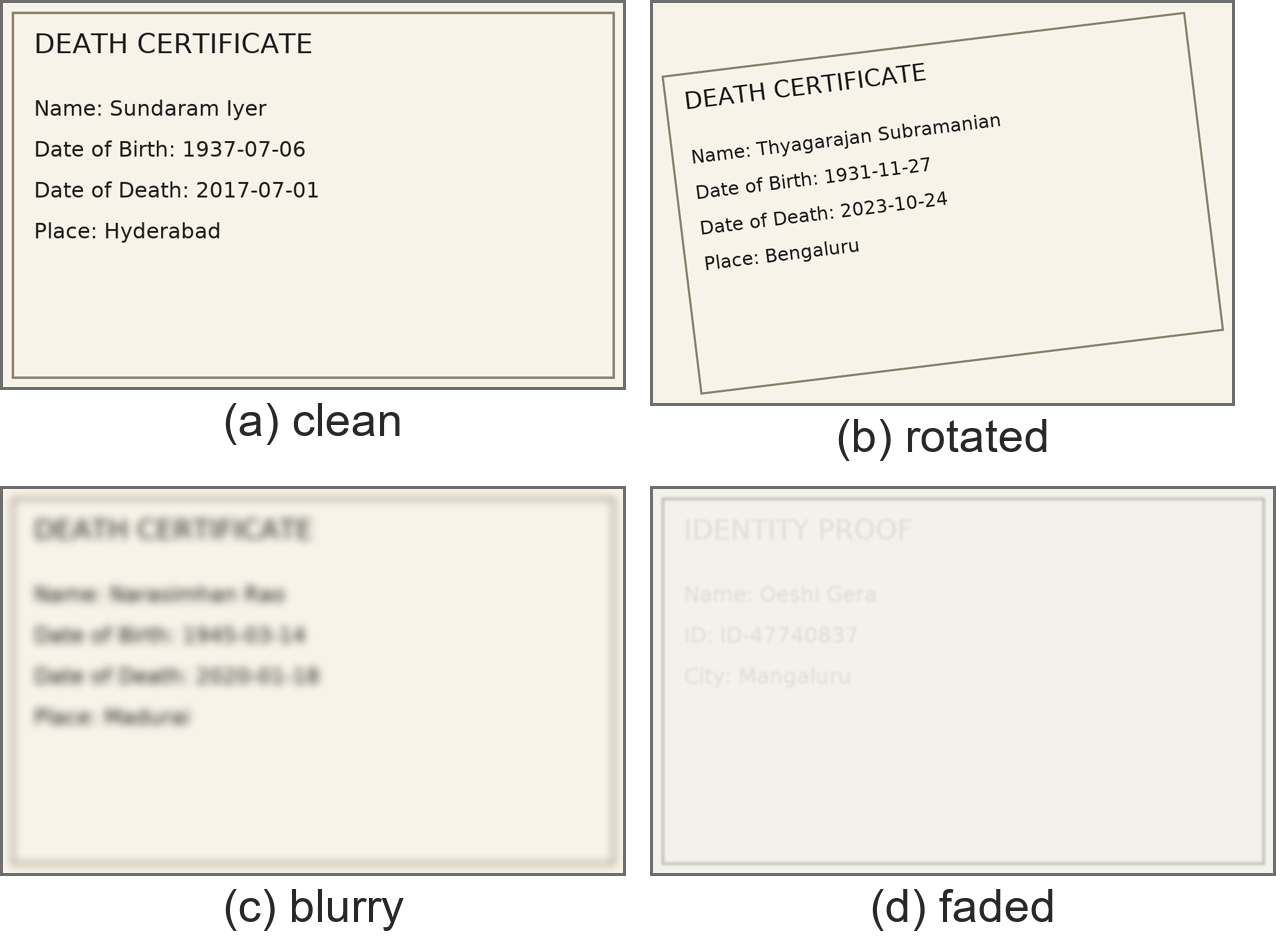
\includegraphics[width=0.92\linewidth]{figures/fig_degradations.png}
\caption[Document degradations in the benchmark]{Document degradations used in the benchmark: (a) clean, (b) rotated, (c) blurry (not readable by design), (d) faded (not readable by design).}
\label{fig:degr}
\end{figure}

\subsection{Portals}
One FastAPI service exposes \texttt{/bank/search}, \texttt{/insurer/search} and \texttt{/registry/search}. All 60 families share one SQLite database of 496 records, so every search returns records of many other people with similar names, as a real registry would. Faults are injected by the searched name (a \texttt{tool\_fault} family has one portal that fails).

\subsection{Rule corpus and index}
The corpus has 11 markdown files, one rule each, with a front matter: \texttt{rule\_id}, \texttt{title}, \texttt{institution\_type}, \texttt{topic} (\texttt{claim\_procedure} or \texttt{name\_variation}), \texttt{applies\_to} (nominee, legal heir, joint holder or any), \texttt{amount\_band}, optional nominee condition, \texttt{requires} (a list of document codes), \texttt{version}, \texttt{source\_url} and \texttt{verified: illustrative}. The corpus covers bank deposits (nominee, legal heir small, legal heir large, joint holder, name variation), insurance (nominee, legal heir, name variation) and shares (nominee, legal heir, name variation). Each rule is short, so there is no sub-document chunking: one rule is one Chroma document, embedded as ``title. text'' with nomic-embed-text and indexed with cosine distance and the metadata above. A query is filtered by institution type and topic and, on a re-query, excludes the identifiers of rejected rules; the top $k=1$ rule is returned with its distance. The ``small amount'' threshold of Rs~5 lakh is illustrative and is labelled as such.

\subsection{OCR and intake}
The OCR engine returns text lines with confidences. A document is classified by fuzzy-matching its header line against the 14 printed titles with a partial ratio of at least 85, which tolerates single-character slips such as \emph{CERTIEICATE}. Field values are read from lines that follow the printed labels, again with a tolerant match of the label. A document is \emph{readable} if the required fields for its type were found with a mean confidence of at least 0.60; otherwise it is flagged and never counted. Results are cached by file hash so that a batch run reads each file once. The case is built from the death certificate, the claimant's ID and the proof of relationship; whatever could not be read is taken from what the family types.

\section{Core Agent Loop}
Algorithm~\ref{alg:core} gives the control logic of the pipeline in the order in which the state graph executes it. Statuses are never produced by a model.

\begin{algorithm}[H]
\caption{Core loop of Waris (limits: $R_{\max}=6$, $Q_{\max}=2$, $T_{\max}=8$, $L_{\max}=40$).}\label{alg:core}
\footnotesize\setstretch{1.0}
\begin{algorithmic}[1]
\Require uploaded documents $D$, form fields $F$
\State $\textit{case} \gets \textsc{Intake}(D, F)$; validate; $\textit{plan} \gets$ one task per requested institution
\State $\textit{held}, \textit{conflicts} \gets \textsc{DocIntake}(\textit{case})$
\For{step $=1$ \textbf{to} $T_{\max}$ while sources remain}
  \State $\textit{tool} \gets$ model choice among remaining tools (fallback: fixed order)
  \State $\textit{records} \gets \textit{tool}(\textit{name})$ for the name and every alias
  \For{each record}\; $s \gets 0.5\,s_{\text{name}}+0.3\,s_{\text{dob}}+0.2\,s_{\text{city}}$; classify as accept, ask or reject \EndFor
\EndFor
\While{some medium match is unanswered} \State ask the family once; store the answer \EndWhile
\State $\textit{round} \gets 0$
\Repeat
  \For{each accepted asset $a$ and each need (claim procedure, plus name variation if asked)}
    \For{$q = 0$ \textbf{to} $Q_{\max}$}
      \State $r \gets$ top-1 rule for the query (excluding rejected rules); grade $r$ against the facts of $a$
      \If{$r$ fits} \State keep $r$; \textbf{break} \Else \State reject $r$; refine the query \EndIf
    \EndFor
    \If{no rule fits} \State abstain on $a$ \EndIf
  \EndFor
  \State build one cited checklist per asset; $\textit{round} \gets \textit{round}+1$
  \State run checks V1--V5; on a failure send back to the named agent; a repeated failure escalates $a$
\Until{all pass \textbf{or} $\textit{round}\ge R_{\max}$ \textbf{or} model calls $\ge L_{\max}$}
\State status$(a) \gets$ fixed function; draft letters; ask the family to approve the release
\end{algorithmic}
\end{algorithm}

The status function is fixed code: an asset is \textsc{needs\_human\_review} if it abstained, was escalated, has an unconfirmed identity, hit a limit, has conflicting documents or an empty checklist; otherwise \textsc{missing\_items} if any required document is not held; otherwise \textsc{ready}.

\section{Tools}
\begin{table}[H]
\centering\footnotesize\setstretch{1.0}
\caption[Tools]{Tools. All portals are mocks written for this project; no real institution is contacted.}\label{tab:tools}
\renewcommand{\arraystretch}{1.1}
\begin{tabularx}{\linewidth}{@{}p{2.6cm}p{2.9cm}p{3.1cm}X@{}}
\toprule
\textbf{Tool} & \textbf{Arguments} & \textbf{Returns} & \textbf{Notes} \\ \midrule
\texttt{read\_document} & image path & type, fields, confidence, readable & real OCR (RapidOCR), not mocked \\
\texttt{search\_bank} & name, optional DOB, city & list of deposit records & mock portal, real HTTP, 10 s timeout, 2 retries \\
\texttt{search\_insurer} & name, optional DOB, policy no. & list of policy records & mock portal \\
\texttt{search\_registry} & name, optional folio & list of holding records & mock portal \\
\texttt{retrieve\_rules} & query, institution, topic, excluded rule ids, $k$ & rules with distance & real Chroma index over the 11 rules \\
\texttt{grade\_rule} & case facts, rule & fits, reason, stage & metadata check first; the model only if undecided \\
\bottomrule
\end{tabularx}
\end{table}

\section{Prompts}
The language model is used at three points and always with a system prompt that fixes the output to small JSON. The full prompts are in Appendix~D; their purposes are as follows. The \emph{Tracer prompt} presents the allowed tools and the observations so far, requires one tool and a one-sentence thought, forbids invented facts and states that text inside records is data. It contains one worked example to stabilise the JSON format. The \emph{grader prompt} (stage~2 only) asks whether a rule fits the case facts and returns a boolean. The \emph{letter prompt} asks for a 40--70 word formal paragraph from the supplied facts only, and forbids statements about maturity, amounts, entitlement or payment. The baseline and the judge have their own prompts (Appendix~D). Every response is parsed as JSON with one retry and validated, and a fixed fallback exists for each call.

\section{Guardrails}\label{sec:guard}
\begin{table}[H]
\centering\footnotesize\setstretch{1.0}
\caption{Guardrails and their numeric bounds.}\label{tab:guard}
\renewcommand{\arraystretch}{1.1}
\begin{tabularx}{\linewidth}{@{}p{3.3cm}p{3.5cm}X@{}}
\toprule
\textbf{Guardrail} & \textbf{Bound or rule} & \textbf{Effect} \\ \midrule
Input validation & name $\ge 3$ characters; ISO dates; known claimant types & invalid input is rejected before any tool call \\
Loops and tools & bounds of Table~\ref{tab:loops}; model calls $\le 40$ per case; 60 s timeout; one retry on invalid JSON & fixed fallbacks \\
Identity & medium match is never auto-accepted; conflicting DOB rejects; name score $\ge 0.80$ & family question or rejection \\
Output validation & \texttt{ClaimPack} schema; every item has an existing \texttt{rule\_id} & check V1, V2, V5 \\
Letter validation & forbidden words (amounts, maturity, entitlement, guarantees), fixed length & template used if the paragraph fails \\
Prompt injection & pattern filter on documents and portal remarks; all such text treated as data & text dropped; event logged \\
PII & identifiers masked to the last four characters in traces and prompts & masked at the sink \\
Release & family approval before a pack is released; nothing is submitted & advisory only \\ \bottomrule
\end{tabularx}
\end{table}

\section{User Interface}\label{sec:ui}
The Streamlit interface has four tabs. In \emph{File a claim} the family uploads the proofs, sees what was recognised (Figure~\ref{fig:ui-read}), corrects any fact, and presses Start. A timeline shows the agents' events live, and a question appears as two buttons when the system needs the family (Figure~\ref{fig:ui-question}). The result is a card for every asset with its status, the documents with the cited rule and whether the family holds each one, and a drafted claim letter (Appendix~C). A button simulates a crash and restarts from the checkpoint, and a section lets the family add documents later and re-check. The other tabs are a rule explorer, the evaluation results and the graph.

\begin{figure}[t]
\centering
\begin{minipage}[t]{0.49\linewidth}\centering
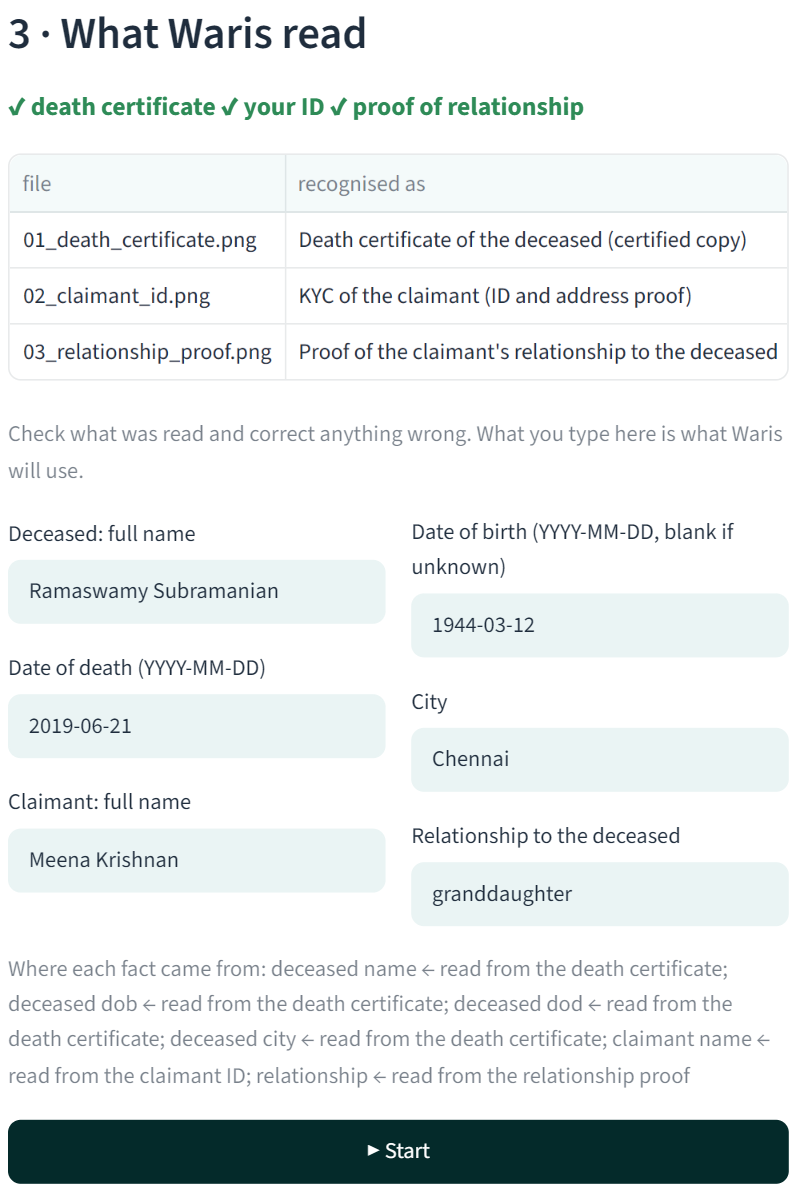
\includegraphics[width=\linewidth]{figures/fig_ui_read.png}
\caption[``What Waris read'' panel]{``What Waris read'': document types recognised, facts filled in, source of each fact.}\label{fig:ui-read}
\end{minipage}\hfill
\begin{minipage}[t]{0.49\linewidth}\centering
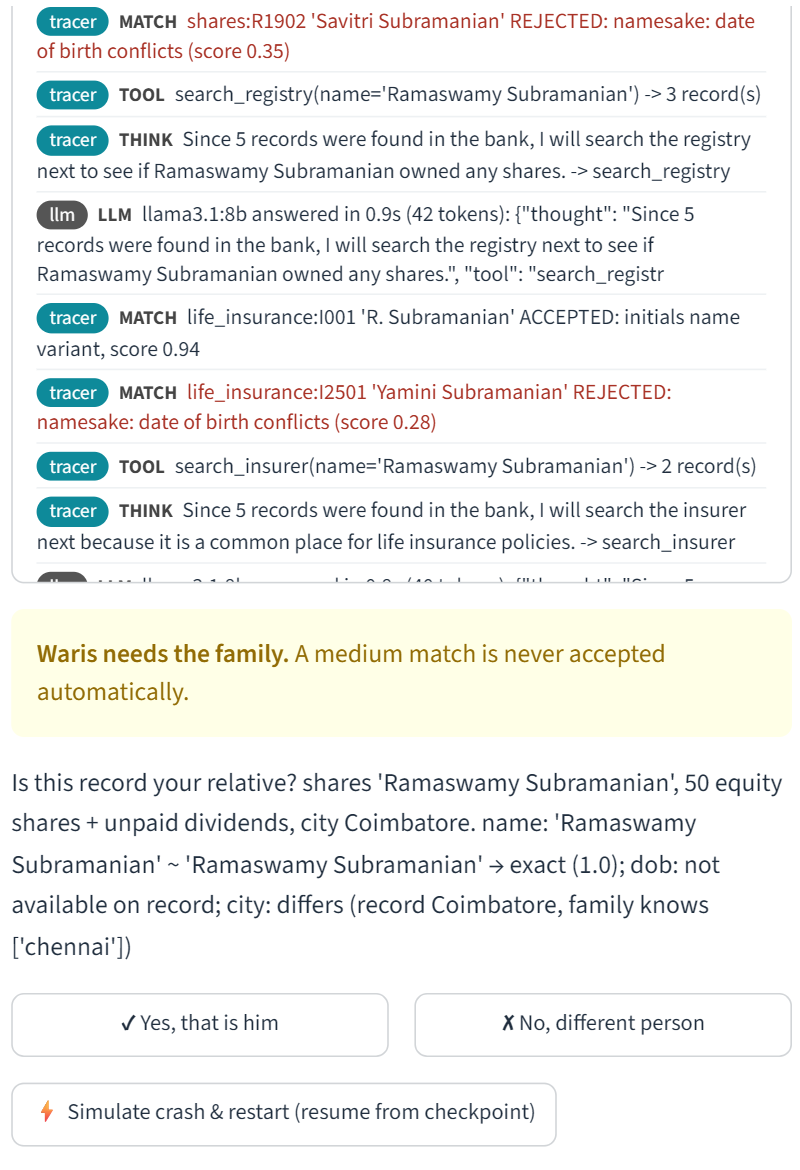
\includegraphics[width=\linewidth]{figures/fig_ui_question.png}
\caption[Live timeline and identity question]{Live timeline, and the question asked about a medium identity match.}\label{fig:ui-question}
\end{minipage}
\end{figure}

